\StartPlate{V07}{Depth can make native trace one invisible}{The valuation inequality is the mechanism, not an assertion that the trace is zero.}
\begin{center}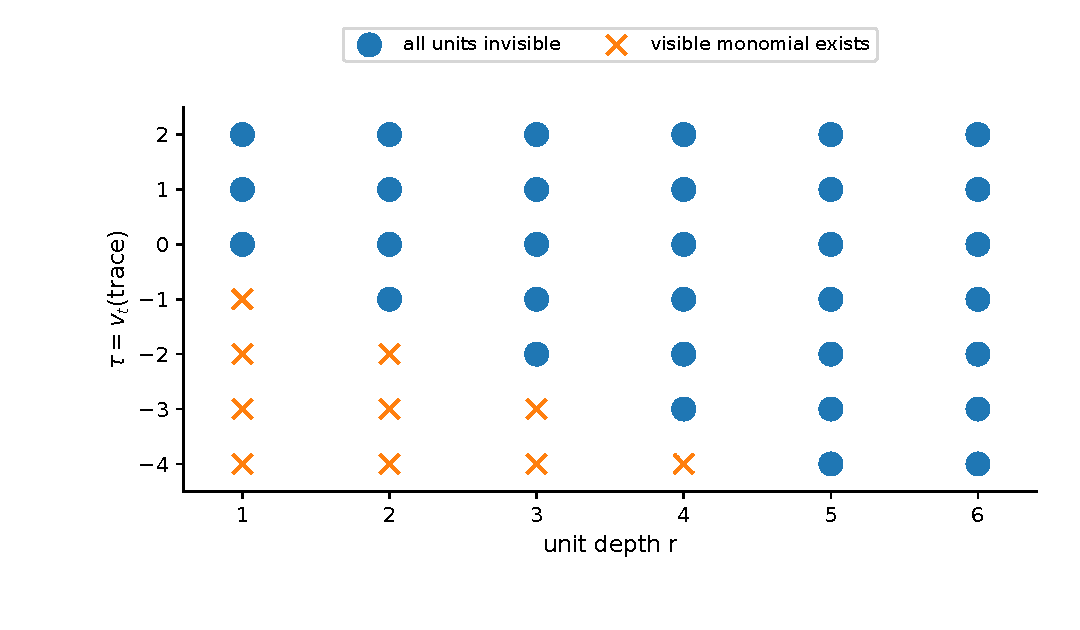
\includegraphics[width=\linewidth]{figures/V07.pdf}\end{center}
In $\F_2((t))$, let the additive character read the coefficient of $t^0$. Model the trace coefficient by $t^\tau$, and let the variable range over $t^r\mathcal O$. A circle means every such product has positive valuation and is invisible to the character:
\[
\tau+r\ge1.
\]
At a cross, $t^{-\tau}$ belongs to the allowed domain and produces the visible product $1$. This gives an explicit negative control, rather than treating failure of a sufficient bound as proof of visibility without a witness.

The native trace-one row is $\tau=0$. It is invisible at every positive unit depth in the displayed range. Native trace one, zero trace after amplification, and the trace of the correction remain different quantities in the arithmetic recursion. The exact floor in the correction depth is retained in the written proof. This monomial picture explains the inequality but does not replace the full shallow-character extension argument.
\vfill\PlateSource{Exact Laurent-monomial model}{Part I, Section 8}{18}
